\documentclass[a4paper,french,bookmarks]{article}

\usepackage{./Structure/4PE18TEXTB}

\newboxans
\usepackage{booktabs}

\begin{document}

    \renewcommand{\thesection}{\Roman{section}}
    \setlist[enumerate]{font=\color{white5!60!black}\bfseries\sffamily}
    \renewcommand{\labelenumi}{\thesection.\arabic{enumi}.}
    \renewcommand*{\labelenumii}{\thesection.\arabic{enumi}.\arabic{enumii}.}
    
    \stylizeDocSpe{Physique}{Devoir maison n° 2}{}{Pour le mercredi 21 septembre 2022}
    
    \section{Premier problème}
    
    On considère un filtre d'ordre $2$ inconnu. O, redonne les fonctions de transfert envisagées :
    %
    \[ \underline{H}_1 = \frac{-\p{\frac{\omega}{\omega_0}}^2G_0}{1 - \p{\frac{\omega}{\omega_0}}^2 + \jj\frac{\omega}{Q\omega_0}} \qquad\qquad \underline{H}_2 = \frac{G_0}{1 + \jj Q\p{\frac{\omega}{\omega_0} - \frac{\omega_0}{\omega}}} \qquad\qquad \underline{H}_3 = \dfrac{G_0}{1 - \p{\frac{\omega}{\omega_0}}^2 + \jj\frac{\omega}{Q\omega_0}}\]
    %
    On donne deux oscillogrammes pour deux fréquences du signal d'entrée (créneau, \texttt{voie A}) différentes. Le signal en \texttt{voie B} est la tension de sortie du filtre.
    
    \begin{center}
        \begin{minipage}{0.95\linewidth}
            \begin{minipage}{0.48\linewidth}
                \begin{center}
                    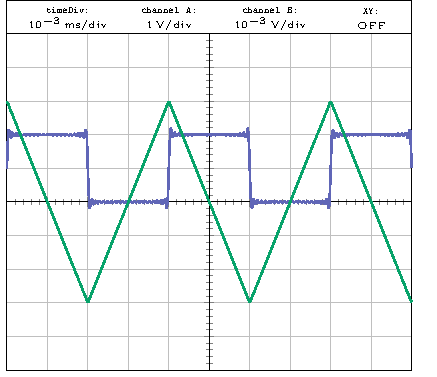
\includegraphics{Figures/MPIPHDM2F1.pdf}
                \end{center}
            \end{minipage}
            %
            \hfill
            %
            \begin{minipage}{0.48\linewidth}
                \begin{center}
                    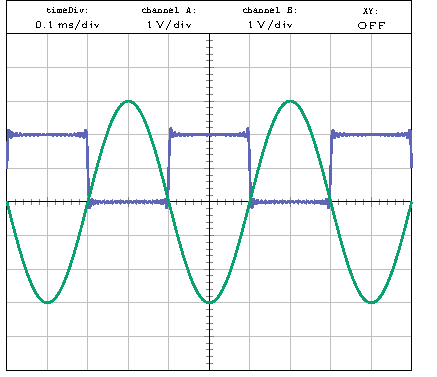
\includegraphics{Figures/MPIPHDM2F2.pdf}
                \end{center}
            \end{minipage}
        \end{minipage}
    \end{center}
    
    On fournit la décomposition en série de \textsc{Fourier} des signaux triangulaires et créneaux d'amplitude $V_0$ :
    %
    \[ s_\text{tr}\p{t} = \dfrac{8V_0}{\pi} \sum_{p=0}^{+\infty} \p{-1}^p \dfrac{\sin\p{\p{2p + 1}\omega_1 t}}{\p{2p + 1}^2}\qquad s_\text{cr}\p{t} = \dfrac{4V_0}{\pi} \sum_{p=0}^{+\infty} \dfrac{\sin{\p{2p + 1}\omega_1t}}{2p + 1}\]
    
    \begin{enumerate}
        \item Décrire l'effet du filtre sur le signal d'entrée pour les deux fréquences présentées.
        
        \boxansconc{
            \begin{enumerate}
                \itt On remarque premièrement que dans la figure de gauche comme de droite, la composante continue du signal d'entrée (signal créneau en \texttt{voie A}) est de valeur $\SI{1}{\volt}$, donc non nulle. Or la composante continue du signal de sortie est nulle dans les deux cas, elle a donc été coupée.
                
                \itt Par ailleurs, le signal de gauche est de période $T_g = \SI{4e-3}{\milli\second}$, donc de fréquence $f_g = \frac{1}{T_g} \approx \SI{250}{\kilo\hertz}$. Celui de droite est de période $T_d = \SI{4e-1}{\milli\second}$ donc de fréquence $f_d = \SI{2.5}{\kilo\hertz}$. Or le signal de gauche est d'amplitude crête à crête $A_g = \SI{6}{\milli\volt}$ et celui de droite d'amplitude crête à crête $A_d = \SI{6}{\volt}$, donc $A_d \gg A_g$. Les hautes fréquences sont donc coupées, ce qui est corroboré par la disparition des discontinuités (harmoniques de haute fréquences) sur le signal de droite.
                
                \itt On observe également que le signal de sortie gauche (haute fréquence) est un signal triangle, qu'on peut voir comme une primitive du signal créneau en entrée (\cf formules ci-dessus). On a donc un comportement intégrateur. 
            \end{enumerate}
            
        }
        
        \item En déduire la nature du filtre et la fonction de transfert associé. Évaluer sa fréquence propre $f_0$.
        
        \noafter
        %
        \boxans{
            Le filtre coupe les hautes fréquences et a un comportement intégrateur, ainsi on pourrait envisager un passe 
        }
        %
        \nobefore
        %
        \boxansconc{
            bas. Cependant, la composante continue est aussi éliminée, donc le filtre semble plutôt être un passe bande.
        }
        %
        \boxans{
            Pour $\omega$ très grand (donc à haute fréquence), on a $\underline H_1 \asymp{\omega \to +\infty} G_0$ donc ce n'est pas $\underline H_1$.
            
            Pour $\omega$ très petit (donc à basse fréquence), on a $\underline H_3 \asymp{\omega \to 0} G_0$ donc ce n'est pas non plus $\underline H_3$.
        }
        %
        \boxansconc{
            Par élimination, la fonction de transfert du filtre est $\underline H = \underline{H}_2 = \dfrac{G_0}{1 + \jj Q\p{\frac{\omega}{\omega_0} - \frac{\omega_0}{\omega}}} = \dfrac{G_0}{1 + \jj Q\p{\frac{f}{f_0} - \frac{f_0}{f}}}$.
        }
        %
        \boxans{
            On établi l'expression du gain $G = \mod{\underline H}$ en fonction de $f$ :
            %
            \[ G\p{f} = \mod{\underline H} = \mod{\dfrac{G_0}{1 + \jj Q\p{\frac{f}{f_0} - \frac{f_0}{f}}}} = \dfrac{G_0}{\mod{1 + \jj Q\p{\frac{f}{f_0} - \frac{f}{f_0}}}} = \dfrac{G_0}{\sqrt{1 + Q^2\p{\frac{f}{f_0} - \frac{f_0}{f}}^2}}\]
            %
            %Donc
            %
            %\[ 1 + Q^2\p{\frac{f}{f_0} - \frac{f_0}{f}}^2 = \p{\dfrac{G_0}{G\p{f}}}^2 \quad \text{donc} \quad \frac{f}{f_0} - \frac{f_0}{f} = \frac{1}{Q}\sqrt{\dfrac{{G_0}^2}{G\p{f}^2} - 1} \quad \text{donc} \quad {f_0}^2 + \frac{f}{Q}\sqrt{\dfrac{{G_0}^2}{G\p{f}^2} - 1}f_0 - f^2 = 0\]
            %
            %Les solutions sont donc de forme (on prend la solution positive car $f \geq 0$) :
            %
            %\[ f_0 = \dfrac{-\frac{f}{Q}\sqrt{\frac{{G_0}^2}{G\p{f}^2} - 1} + \sqrt{\frac{f^2}{Q^2}\p{\frac{{G_0}^2}{G\p{f}^2} - 1} + 4f^2}}{2} = \dfrac{f}{2Q}\p{\sqrt{\frac{{G_0}^2}{G\p{f}^2} - 1 + 4Q^2}-\sqrt{\frac{{G_0}^2}{G\p{f}^2} - 1}}\]
            %
            \begin{enumerate}
                \itt Pour l'oscillogramme de gauche, on a $f_g = \SI{250}{\kilo\hertz}$ et une amplitude crête à crête de sortie de $A_g = \SI{6}{\milli\volt}$. Or le signal d'entrée est d'amplitude crête à crête $A_e = \SI{4}{\volt}$ donc $G\p{f_g} = \frac{A_g}{A_e} = \SI{1.5e-3}{}$.
                
                \itt Pour l'oscillogramme de droite, on a $f_d = \SI{2.5}{\kilo\hertz}$ et une amplitude crête à crête de sortie de $A_d = \SI{6}{\volt}$. Or le signal d'entrée est d'amplitude crête à crête $A_e = \SI{4}{\volt}$ donc $G\p{f_d} = \frac{A_d}{A_e} = \SI{1.5}{}$.
            \end{enumerate}
            %
            \[ \dfrac{G\p{f_d}}{G\p{f_g}} = \dfrac{\frac{G_0}{\sqrt{1 + Q^2\p{\frac{f_d}{f_0} - \frac{f_0}{f_d}}^2}}}{\frac{G_0}{\sqrt{1 + Q^2\p{\frac{f_g}{f_0} - \frac{f_0}{f_g}}^2}}} = \sqrt{\dfrac{1+Q^2\p{\frac{f_g}{f_0} + \frac{f_0}{f_g}}^2}{1 + Q^2\p{\frac{f_d}{f_0} + \frac{f_0}{f_d}}^2}}\]
            %
            Or $f_0$ est indépendante de $Q$, donc en prenant $Q \to +\infty$ dans la formule ci-dessus, on obtient :
            %
            \[ \dfrac{G\p{f_d}}{G\p{f_g}} = \dfrac{\frac{f_g}{f_0} - \frac{f_0}{f_g}}{\frac{f_d}{f_0} - \frac{f_0}{f_d}} \qquad\text{donc}\qquad \dfrac{G\p{f_d}}{G\p{f_g}} = \dfrac{f_g-\frac{1}{f_g}{f_0}^2}{f_d - \frac{1}{f_d}{f_0}^2} \qquad\text{donc}\qquad \dfrac{G\p{f_d}}{G\p{f_g}}f_d - f_g = \p{\dfrac{G\p{f_d}}{G\p{f_g}f_d} - \dfrac{1}{f_g}}{f_0}^2\]
            %
            On a donc ${f_0}^2 = \dfrac{\frac{G\p{f_d}}{G\p{f_g}}f_d - f_g}{\frac{G\p{f_d}}{G\p{f_g}f_d} - \frac{1}{f_g}} = \dfrac{\phantom{r}\frac{G\p{f_d}f_d - G\p{f_g}f_g}{G\p{f_g}}\phantom{r}}{\frac{G\p{f_d}f_g - G\p{f_g}f_d}{G\p{f_g}f_df_g}} = f_df_g\dfrac{G\p{f_d}f_d - G\p{f_g}f_d}{G\p{f_d}f_g - G\p{f_g}f_d}$.
        }
        %
        \yesafter
        %
        \boxansconc{
            Puisque $f_0 \geq 0$, on a $f_0 = \sqrt{f_df_g\dfrac{G\p{f_d}f_d - G\p{f_g}f_d}{G\p{f_d}f_g - G\p{f_g}f_d}}$. L'application numérique livre $f_0 \approx \SI{2.4}{\kilo\hertz}$.
        }
        %
        \yesbefore
        
        \item Tracer le diagramme de \textsc{Bode} du filtre.
        
        On prendra, \textbf{pour cette question uniquement}, $Q = 10^3$ et $G_0 = 0,1$.
        
        \boxansconc{
            On trace les diagrammes en fonction de la pulsation réduite $x = \frac{\omega}{\omega_0} = \frac{f}{f_0}$ et selon les expressions :
            %
            \[ G_\text{dB}\p{x} = 20\log{G\p{x}} = -20\log{1 + 10^6\p{x - \frac{1}{x}}^2} \qquad\qquad \varphi\p{x} = \arg{\underline H\p{x}} = -\arctan{10^3\p{x - \frac{1}{x}}}\]
            
            \begin{minipage}{0.50\linewidth}
                \begin{center}
                    \underline{Diagramme en gain :}\newline\text{}
                    
                    \begin{tikzpicture}
                    \begin{axis}[
                        xmode               =   log,
                        axis lines          =   left,
                        domain              =   0.001:1000,
                        xmin                =   0.001,
                        xmax                =   1000,
                        ymin                =   -200,
                        ymax                =   10,
                        grid                =   both,
                        width               =   8cm,
                        height              =   5.5cm,
                        legend pos          = north east,
                        legend style={row sep=0.1cm, font=\scriptsize}
                        ]               
                            \addplot[color=main3,samples=500,smooth,thick]{-20-10*ln(1+1000000*(x-1/x)^2)/ln(10)};
                            \legend{$x \mapsto G_\text{dB}\p{x}$}
                        \end{axis}
                    \end{tikzpicture}
                \end{center}
            \end{minipage}
            %
            \begin{minipage}{0.50\linewidth}
                \begin{center}
                    \underline{Diagramme en phase :}\newline\text{}
                    
                    \begin{tikzpicture}
                    \begin{axis}[
                        xmode               =   log,
                        axis lines          =   left,
                        domain              =   0.1:10,
                        xmin                =   0.1,
                        xmax                =   10,
                        ymin                =   -2,
                        ymax                =   2,
                        grid                =   both,
                        width               =   8cm,
                        height              =   5.5cm,
                        ytick               = {-pi/2, 0, pi/2},
                        yticklabels         = {$-\sfrac{\pi}{2}$, $0$, $\sfrac{\pi}{2}$},
                        legend pos          = north east,
                        legend style={row sep=0.1cm, font=\scriptsize}
                        ]               
                            \addplot[color=main3,samples=3000,smooth,thick]{rad(-atan(10^3*(x-1/x)))};
                            \legend{$x \mapsto \varphi\p{x}$}
                        \end{axis}
                    \end{tikzpicture}
                \end{center}
            \end{minipage}
            }
        
        \item A l'aide du deuxième oscillogramme, évaluer $G_0$.
        
        \boxansconc{
            On a $f_d \approx f_g$ d'où $G\p{f_d} \approx \dfrac{G_0}{\sqrt{1 + 0^2}}$ d'où $G_0 = G\p{f_d} = 1.5$.
        }
        
        \item A l'aide du premier oscillogramme, évaluer $Q$.
        
        \boxansconc{
            On a $G\p{f_g} = \dfrac{G_0}{\sqrt{1+Q^2\p{\frac{f_g}{f_0} + \frac{f_0}{f_g}}^2}}$ d'où $Q = \dfrac{\sqrt{\frac{{G_0}^2}{G\p{f_g}^2} - 1}}{\frac{f_g}{f_0} + \frac{f_g}{f_0}}$. L'application numérique donne $Q \approx \SI{10}{}$.
        }
        
    \end{enumerate}
    
    \section{Deuxième problème}
    
    Un circuit est constitué d'une bobine idéale d'autoinductance $L$, un condensateur de capacité $C$, initialement déchargé, et une résistance $R$ formant deux dipôles $D_1$ et $D_2$ connectés en série avec un générateur de tension continue $E = \SI{15}{\volt}$. En régime permanent le circuit est parcouru par un courant $I = \SI{15}{\milli\ampere}$.
    
    Le régime transitoire de la tension $u\p{t}$ aux bornes de $D_2$ est donné par le chronogramme ci-dessous ($t = \SI{0}{\second}$ est l'instant où l'on a fermé un interrupteur entre le générateur et les dipôles) :
    
    \begin{center}
        \begin{tikzpicture}
            \begin{axis}[
                axis lines          =   middle,
                axis line style     =   {-stealth,shorten >=-3mm},
                domain              =   0:13,
                xmin                =   0,
                xlabel              =   $t$,
                ylabel              =   $u\p{t}$,
                every axis x label/.style={
                    at      =   {(xticklabel cs:1,0)},
                    yshift  =   1.8em,
                    anchor  =   south west
                },
                every axis y label/.style={
                    at      =   {(yticklabel cs:1,0)},
                    xshift  =   3.7em,
                    yshift  =   0.1em,
                    anchor  =   south east
                },
                xmax                =   13,
                ymin                =   -9,
                xtick distance      =   1,
                ytick distance      =   1,
                ymax                =   9,
                grid                =   major,
                width               =   12cm,
                height              =   7cm,
                ytick               =   {},
                yticklabels         =   {}
            ]               
                \addplot[color=main3,samples=300,smooth,thick]{-9.5*(exp(-x/2.3)*cos(180*(4/3*x+1/2)))};
            \end{axis}
        \end{tikzpicture}
    \end{center}
    
    \begin{enumerate}
        \item Déterminer de quoi sont constitués les dipôles $D_1
        $ et $D_2$. Faire un schéma du circuit.
        
        \noafter
        \boxans{
            \begin{minipage}{0.48\linewidth}
                En régime permanent ($t \to +\infty$), le condensateur agît comme un interrupteur ouvert. Supposons que le générateur, la résistance, le condensateur et la bobine soient tous en série (circuit $RLC$ ci-contre). On aurait donc $i\p{t} \lima{t \to +\infty} 0$, ce qui n'est pas le cas.
            \end{minipage}
            %
            \hfill
            %
            \begin{minipage}{0.5\linewidth}
                \begin{center}
                    \begin{circuitikz}
                        \draw (0, 0) to[vsource, v=$E\p{t}$] ++(0, 2) --++(0.5, 0) to[R, l=$R$, v=$u_R\p{t}$] ++(2, 0) --++(0.5, 0) to[L, l=$L$, v=$u_L\p{t}$] ++(2, 0) --++(0.5, 0) to[C, l=$C$, v=$u_E\p{t}$] ++(0, -2) to[short, i_=$i\p{t}$, -*] ++(-4, 0) --++(-0.35, 0.35);
                    
                        \draw (0, 0) to[short, -o] ++(1, 0);
                    \end{circuitikz}
                \end{center}
            \end{minipage}
            
            \text{}\newline\newline
            
            \begin{minipage}{0.38\linewidth}
                Or les dipôles $D_1$ et $D_2$ sont en série, et puisqu'il y a forcément un composant dans $D_1$ et $D_2$, on en déduit que le circuit est de la forme ci-contre.
            \end{minipage}
            %
            \hfill
            %
            \begin{minipage}{0.6\linewidth}
                \begin{center}
                    \begin{circuitikz}
                        \draw (0, 0) to[vsource, v=$E\p{t}$] ++(0, 2) --++(1, 0) to[R, name=D1, v=$u_{D_i}\p{t}$] ++(2, 0) --++(1.7, 0) to[C, l_=$C$, v^=$u_C\p{t}$] ++(0, -2) to[short, -*, i_=$i\p{t}$, -*] ++(-3.2, 0) --++(-0.35, 0.35);
                        
                        \draw (4.7, 2) --++(1.7, 0) to[R, name=D2] ++(0, -2) --++(-1.7, 0);
                        
                        \node at (D1.center) {$L$ ou $R$};
                        \node[rotate=-90] at (D2.center) {$L$ ou $R$};
                    
                        \draw (0, 0) to[short, -o] ++(1, 0);
                        
                        \draw[dashed] (0.5, 2.6) -- (0.5, 1.2) -- (3.5, 1.2) -- (3.5, 2.6) --node[fill=main1white2!50!gray!7] {$D_i$} (0.5, 2.6) ;
                        
                        \draw[dashed] (3.8, 2.6) -- (3.8, -0.3) -- (6.8, -0.3) -- (6.8, 2.6) --node[fill=main1white2!50!gray!6] {$D_j$} (3.8, 2.6) ;
                    \end{circuitikz}
                \end{center}
            \end{minipage}
            %
            \text{}\newline\newline
            %
            En considérant la maille avec le générateur, $D_i$ et le condensateur, on obtient par \textit{loi des mailles }que $E\p{t} = u_{D_i}\p{t} + u_C\p{t}$. Le condensateur étant initialement déchargé, il est équivalent à un fil et donc $u_C\p{0} = 0$. Il en résulte que $u_{D_i}\p{0} = E\p{0} = E \neq 0 = u_{D_2}\p{0}$ donc $D_i = D_1$ et $D_2 = D_j$.\newline
            
            On obtient similairement que $E = u_{D_1} + u_{D_2}$, donc $u_{D_1} = E - u_{D_2}$, et puisque $u_{D_2}\p{t} \lima{t \to +\infty} 0$, on a $u_{D_1}\p{t} \lima{t \to +\infty} E$. Puisqu'une bobine est équivalente en régime permanent à un fil (donc de tension nul), il en résulte que $D_1$ contient forcément la résistance, et $D_2$ la bobine. 
        }
        %
        \nobefore\yesafter
        %
        \boxansconc{
            Le circuit est donc :\newline
            \begin{center}
                    \begin{circuitikz}
                        \draw (0, 0) to[vsource, v=$E\p{t}$] ++(0, 2) --++(1, 0) to[R, l=$R$, v=$u_R\p{t}$] ++(2, 0) --++(1.7, 0) to[C, l_=$C$, v^=$u\p{t}$, i_=$i_1\p{t}$] ++(0, -2) to[short, -*, i_=$i\p{t}$, -*] ++(-3.2, 0) --++(-0.35, 0.35);
                        
                        \draw (4.7, 2) to[short, i=$i_2\p{t}$] ++(1.7, 0) to[L, l_=$L$, v^=$u_L\p{t}$] ++(0, -2) --++(-1.7, 0);
                        
                        \draw (0, 0) to[short, -o] ++(1, 0);
                        
                        \draw[dashed] (0.5, 2.8) -- (0.5, 1.2) -- (3.5, 1.2) -- (3.5, 2.8) --node[fill=main1white2!50!gray!7] {$D_1$} (0.5, 2.8) ;
                        
                        \draw[dashed] (3.8, 2.8) -- (3.8, -0.3) -- (7.7, -0.3) -- (7.7, 2.8) --node[fill=main1white2!50!gray!6] {$D_2$} (3.8, 2.78) ;
                    \end{circuitikz}
                \end{center}
                
                \text{}
        }
        %
        \yesbefore
        
        \item Établir l'équation différentielle vérifiée par $u\p{t}$, la tension aux bornes de $D_2$. La mettre sous la forme de canonique :\qquad  $\dfrac{\dif^2 u}{\dif t^2} + \dfrac{\omega_0}{Q}\dfrac{\dif u}{\dif t} + {\omega_0}^2 u = 0$.
        
        \noafter
        %
        \boxans{
            Par \text{loi des mailles}, on a $E = u_R\p{t} + u\p{t}$. Or par \text{loi d'\textsc{Ohm}} on a $u_R\p{t} = Ri\p{t}$ et par \textit{loi des noeuds} on a $i\p{t} = i_1\p{t} + i_2\p{t}$, d'où $E = R\p{i_1\p{t} + i_2\p{t}} + u\p{t}$. Par \textit{relation constitutive d'un condensateur} on a $i_1\p{t} = C\dfrac{\dif u}{\dif t}$ d'où :
            %
            \[ E = RC\dfrac{\dif u}{\dif t} + Ri_2\p{t} + u\p{t} \qquad\text{donc en dérivant}\qquad RC\dfrac{\dif^2 u}{\dif t^2} + \dfrac{\dif u}{\dif t} + R\dfrac{\dif i_2}{\dif t}\]
            %
            Par \textit{relation constitutive d'une bobine}, on a $u\p{t} = L\dfrac{\dif i_2}{\dif t}$ d'où $\dfrac{\dif i_2}{\dif t} = \dfrac{1}{L}u\p{t}$, donc :
            %
            \[ RC\dfrac{\dif^2 u}{\dif t^2} + \dfrac{\dif u}{\dif t} + \dfrac{R}{L}u\p{t} = 0 \qquad\text{donc}\qquad \dfrac{\dif^2 u}{\dif t^2} + \dfrac{1}{RC}\dfrac{\dif u}{\dif t} + \dfrac{1}{LC}u\p{t} = 0\]
        }
        %
        \nobefore\yesafter
        %
        \boxansconc{
            Donc $u\p{t}$ vérifie l'équation différentielle $\dfrac{\dif^2 u}{\dif t^2} + \dfrac{\omega_0}{Q}\dfrac{\dif u}{\dif t} + {\omega_0}^2 u = 0$ avec $\omega_0 = \dfrac{1}{\sqrt{LC}}$ et $Q = R\sqrt{\dfrac{C}{L}}$.
        }
        %
        \yesafter
        
        \item Estimer une valeur approchée de $Q$ et $\omega_0$ à l'aide du chronogramme, puis en déduire les valeurs de $L$, $R$ et $C$.
        
        \noafter
        %
        \boxans{
            On observe des oscillations dans le régime transitoire, donc on est dans le cas $Q > \sfrac{1}{2}$. En posant $\alpha = \dfrac{\omega_0}{2Q} \neq 0$ le facteur d'amortissement, on a :
            %
            \[ u\p{t} = e^{-\alpha t}\p{A\sin{\omega t} + B\cos{\omega t}} \qquad\text{avec}\quad A \et B \ \text{des constantes à déterminer et} \ \omega = \omega_0\sqrt{1 - \dfrac{1}{4Q^2}}\]
            %
            Or $u\p{0} = 0$ d'où $B = 0$. Puisque en $t = 0$ la bobine agit comme un interrupteur ouvert, on a $i_1\p{0} = i\p{0} = \dfrac{E}{R}$. Or $i_1\p{t} = C\dfrac{\dif u}{\dif t}\p{0} = -CA\alpha\omega$, donc $A = \dfrac{E}{RC\alpha\omega}$.
            %
            \begin{enumerate}
                \itt On sait que dans le cas pseudo-périodique, $Q$ est de l'ordre du nombre d'oscillations visible. On peut donc ici $Q \approx 6 \approx 10$.
                
                \itt On peut déterminer graphiquement la pulsation $\omega $ : la période spatiale est $T = \dfrac{2\pi}{\omega}$ donc $\omega = \dfrac{2\pi}{T}$. On mesure sur le chronogramme sur $\Delta t = \SI{6}{\second}$, environ $4$ périodes, donc $4T = \Delta t$ d'où $T \approx \SI{1.5}{\second}$. On a donc $\omega = \SI{4}{\second^{-1}}$. Puisque $Q$ est grand, on a $\omega \approx \omega_0$ donc $\omega_0 = \SI{4}{\second^{-1}}$.
            \end{enumerate}
            
            On peut donc déterminer les valeurs de $R$, $C$ et $L$. En régime permanent, on a par \textit{loi d'\textsc{Ohm}} que $E = RI$ et donc que $R = \dfrac{E}{I}$. Or on sait que $\dfrac{\omega_0}{Q} = \dfrac{1}{RC}$ d'où $C = \dfrac{Q}{\omega_0R} = \dfrac{IQ}{E\omega_0}$. Enfin, $\omega_0 = \dfrac{1}{\sqrt{LC}}$ d'où $L = \dfrac{1}{C{\omega_0}^2} = \dfrac{E}{IQ\omega_0}$.
        }
        %
        \nobefore\yesafter
        %
        \boxansconc{
            On a donc $R = \SI{1}{\kilo\ohm}$, $C = \SI{1.5}{\micro\farad}$ et $L = \SI{4e1}{\henry}$.
        }
        %
        \yesbefore
    
        \item Tracer l'allure du portrait de phase pour $u\p{t}$. 
        
        \boxansconc{
            \begin{center}
                \begin{tikzpicture}
                    \begin{axis}[
                        axis lines          =   middle,
                        domain              =   0:13,
                        xmin                =   -9,
                        xlabel              =   $u$,
                        ylabel              =   $\dot u$,
                        xmax                =   9,
                        ymin                =   -50,
                        xtick distance      =   1,
                        ytick distance      =   10,
                        ymax                =   50,
                        grid                =   major,
                        width               =   13.5cm,
                        height              =   10cm,
                        ytick               =   {},
                        yticklabels         =   {},
                        xtick               =   {},
                        xticklabels         =   {}
            ]               
                \addplot[color=main3,samples=300,smooth,thick]({-9.5*(exp(-x/2.3)*cos(180*(4/3*x+1/2)))}, {40*(exp(-x/2.3)*sin(180*(4/3*x+1/2)))});
            \end{axis}
        \end{tikzpicture}
            \end{center}
        }
        
    \end{enumerate}
    
\end{document}